\chapter{Embedding Everyday Objects to Augment 3D Prints}

\begin{figure} [h]
	\centering
   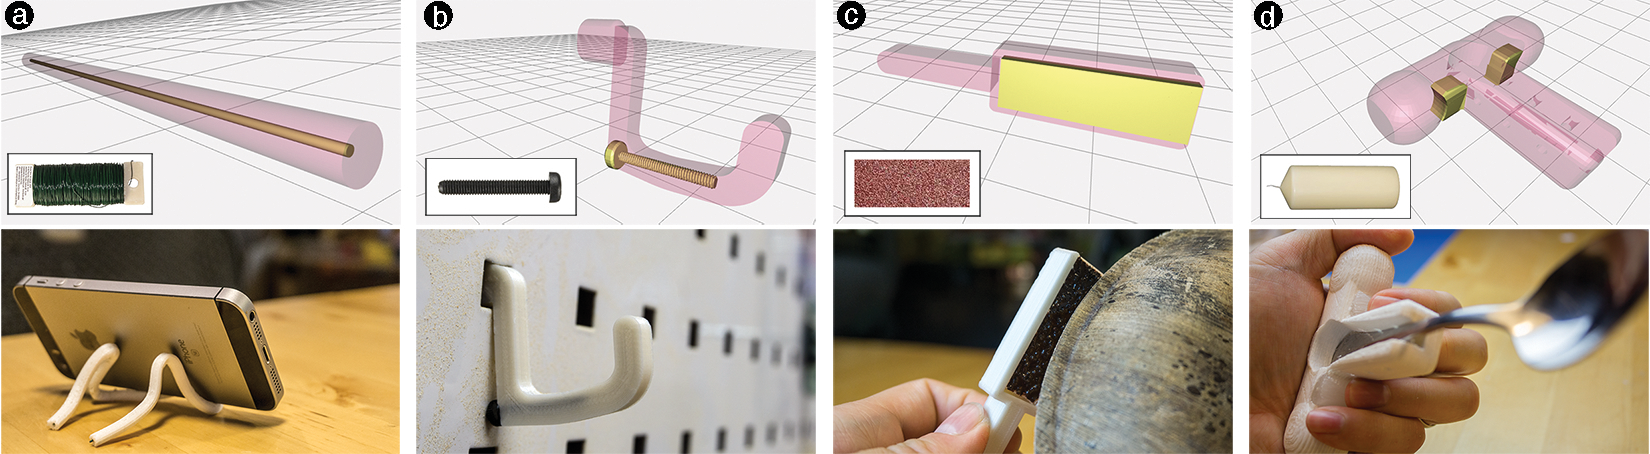
\includegraphics[width=1\textwidth]{figures/fig1}
   \caption{We present a library of \textit{embeddables}---everyday objects that can be cut, worked and embedded into 3D printable designs to augment their material properties. For example, inserting a florists' wire makes elastic TPU-based objects stay in shape (plastic deformation) (a); a screw is used to reinforce a pegboard hook (b); a piece of sand paper becomes the surface of a printed sander (c); the malleability of wax makes it possible to further personalize assistive devices even after they are printed (d).}~\label{fig:fig1}
\end{figure}


The previous three projects focus on augmenting existing real-world objects with 3D printed designs. In this chapter, I flip the relationship and explore how real-world objects can be used to augment 3D printed designs. % Background
In our everyday life, we are surrounded by objects with a wide range of material properties. Consider gloves as an example. They can be made of leather for insulation against cold (Figure~\ref{fig:gloves}a), or silicone for protection against heat (Figure~\ref{fig:gloves}b), or nitrile for elasticity (Figure~\ref{fig:gloves}c), or rubber for better grip and abrasion resistance (Figure~\ref{fig:gloves}d), or even infused with copper to provide support for hands and joints (Figure~\ref{fig:gloves}e).

% Promise & Problem
In contrast, despite the rapid development in multi-material printing, personal fabrication machines (e.g., desktop 3D printers) currently only support a much smaller set of materials. This limits people's creativity in exploring how their designs might incorporate and benefit from various material properties. It also limits the application of fabricated objects, preventing them from being adopted for a wider context of usage.

\begin{figure} [t]
  \centering
  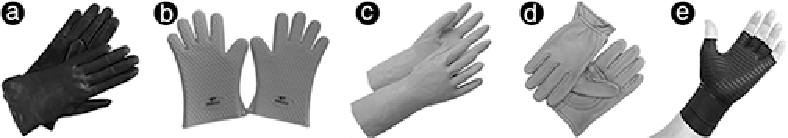
\includegraphics[width=0.75\textwidth]{figures/gloves}
  \caption{Everyday objects are made of various materials, e.g., for gloves, we have leather (a), silicone (b), nitrile (c), rubber (d) and even infused copper (e).}~\label{fig:gloves}
\end{figure}

% State of the art
To overcome the current limitations of material variety, one approach is to design \textit{metamaterials}---a composition of material(s) that exhibits behaviors beyond their natural properties by means of carefully constructed spatial variations in the material(s). Prior work has explored metamaterial designs for elasticity \cite{panetta2015elastic, schumacher2015microstructures}, acoustics \cite{memoli2017metamaterial}, and mechanisms \cite{ion2016metamaterial}. To incorporate an even larger set of properties, another approach is to embed alternate materials, such as conductive paint for interactivity \cite{savage2014series} or state-changeable material for custom deformability \cite{groeger2016hotflex}. Though promising, prior work tends to focus on one or a few specific properties, rather than an approach that affords the exploration of a holistic set.

% Goal
The goal of our research is to leverage a repertoire of material richness in everyday objects to enable the exploration of various material properties in people's custom designs. 
% Technical Solution
To achieve this, we develop a library of \textit{embeddables}---everyday objects that can be cut, worked and embedded into 3D printable designs. For example, as shown in Figure~\ref{fig:fig1}a, by inserting a florists' wire we can make an elastic object's stay in shape (plastic deformation), such as making a phone holder from a `noodle' printed in TPU (Thermoplastic Polyurethane); embedding an M3 20mm screw strengthens a pegboard hook along its overhanging structure (Figure~\ref{fig:fig1}b); embedding a piece of sand paper adds roughness and creates a simple sander (Figure~\ref{fig:fig1}c); embeddables can also be used for assistive devices: embedding wax into an a spoon handle\footnote{Adopted from `The Andrew Fork': \url{https://www.thingiverse.com/thing:1816581}} allows users to sand it to a custom shape where the fingers can grip comfortably (Figure~\ref{fig:fig1}d).

To enable the use of these embeddables into fabricated designs, we first contribute a systematic categorization of both their geometric and material properties. Specifically, we construct a design space (Figure~\ref{fig:design_space}) composed of two dimensions: in terms of geometry, we define \textit{degree of workability} (DOW) to characterize how different embeddables can be worked into user-defined shapes; in terms of material, we introduce an extensible taxonomy of material properties relevant to personal fabrication. Combined, these two dimensions produce a large space of examples making use of embeddables in various usage scenarios. Further, it also serves to unify a number of projects from prior work.

Building upon the design space, we then contribute Medley--a tool for the computational design and fabrication of embeddables into users' custom designs. With Medley, users can import a 3D model, search for embeddables with desired material properties, and interactively edit and integrate their geometry to fit into the original design. Further, Medley also supports the fabrication and embedding process, including instructions for carving or cutting the objects, and generating optimal paths for inserting them.

% Validation
\subsection{Contribution}
To validate the expressiveness of our approach, we showcase a series of examples augmented by embeddables that go beyond the objects' original printed materials. Our main contribution is a library with computational support for the exploration of material properties to augment personal fabrication, closing the gap between its current limitations and the future of multi-material printing.
	
In the remainder of this paper, we first review related work. Next, we present the design space underpinning the construction of our embeddable library as well as the computational design process. We then demonstrate a wide range of printed results, and describe the technical details, which include specifying the geometry of embeddables, finding optimal insertion paths, and generating instructions and templates to guide the embedding process. We close by discussing current limitations and future work.

\begin{figure}
  \centering
  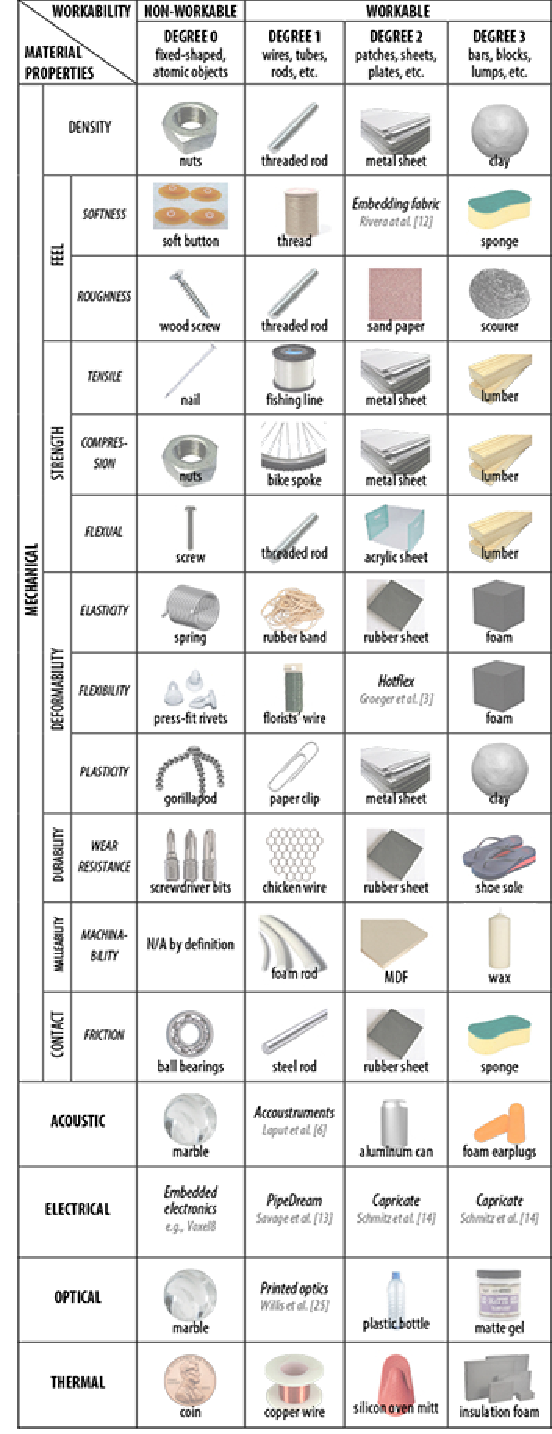
\includegraphics[width=0.5\textwidth]{figures/design_space.pdf}
  \caption{A design space characterizes the material properties of embeddables, as well as their \textit{degree of workability} (DOW)---whether they are embedded as fixed-shape objects (DOW=0), or can be cut to length (1), to a fixed-thickness profile (2), or to a customized 3D form (3).}~\label{fig:design_space}
\end{figure}

% why is it important to consider workability
\section{Design Space}
To design and fabricate objects with embeddables, it is important to understand {\em (i)} material: what properties are available and how to find them in everyday objects, and {\em (ii)} geometric workability: how to work (e.g., cutting, carving) embeddables into specific geometry that fits into certain parts of the design object, which needs to planned at design time as well as executed in the fabrication process. To structure our understanding of these two questions, we construct a design space as shown in Figure~\ref{fig:design_space}. 

The rows of the design space correspond to embeddables' different material properties. These properties are collected from a survey of related work on embedding elements into fabricated objects (shown in italics in Figure~\ref{fig:design_space}) as well as literature in material science \cite{jones2011engineering}. Our current focus is on a set of  material properties that can be found in common everyday objects, and are relevant to personal fabrication (i.e., have been explored in prior work, or can lead to new design directions). Our current list of properties is by no means exhaustive; rather they are meant to be extensible and more properties can be included under this framework.

The columns of the design space describe the embeddables' \textit{degree of workability} (DOW)--how they can be worked into user-defined shape.
 % Specifically, we propose using degree of freedom (DOW) to characterize such workability. 
Notice that DOW is different from the dimension of an embeddable's geometry. For example, as shown below, a wire has DOW 1 (cut to length) yet it can be bent into 2D or 3D geometry.

\begin{itemize}
	\item $DOW=0$ are fixed-shaped, atomic objects that will be directly embedded into a design. For example as shown in Figure~\ref{fig:fig1}b, a screw is embedded into a peg board hook to increase its flexural strength.
	\item $DOW=1$ are wires, tubes or rods of material that can be cut to certain length to create embeddables. Length is the 1 DOW. For example, Figure~\ref{fig:fig1}a shows a florists' wire cut to length and inserted into a TPU-based `noodle' to enable plastic deformation.
	\item $DOW=2$ are patches, sheets or plates of material that can be cut to certain area to create embeddables, thus having 2 DOW on the X/Y plane. The other dimension, thickness, is fixed. For example, a piece of sand paper is cut to replace certain area in order to create a printed sander (Figure~\ref{fig:fig1}c).
	\item $DOW=3$ are bars, blocks or lumps of material that can be cut to arbitrary 3D shape within their size limits. For example, by carving out two pieces of finger-sized wax we can embed them to customize the handle of an assistive utensil holder (Figure~\ref{fig:fig1}d).
\end{itemize}

Each cell in Figure~\ref{fig:design_space} contains one example---either a piece of related work or an embeddable---with the specific material property and DOW. Admittedly each of these is not the only example of a particular cell, or necessarily better than the other examples not shown here. They merely serve to provide a concrete illustration of what embeddables are possible within a given cell, and potentially a starting point for interested readers to explore other similar embeddables. On the other hand, one embeddable might have more than one property relevant to fabrication. For example, an embeddable might exhibit a similar set of properties, such as lumber has nice tensile, compressive and flexural strengths; in other cases, one embeddable might present quite different properties, such as kitchen sponge is both soft and has high surface friction due to its porousness.



\section{A Library of Embeddables $\mathbf{\rightarrow}$ Rich Materiality}
% - showing library on the ui
Based on the design space, we have constructed an extensible library of embeddables. To validate its expressiveness, in this section, we first demonstrate results showing how this library enables the exploration of rich material properties in 3D printed objects. We leave the technical details in the next few sections where we then describe how to computationally design with embeddables from the library.

 % integrated into Medley--a computational tool for specifying, generating and inserting embeddables into a 3D design. 

It is beyond the scope of this paper to include every single cell in Figure~\ref{fig:design_space}; rather, our strategy is to create a set of examples that sample broadly across the design space. In so doing, our goal is to validate how this space holistically affords the enabling of rich material properties beyond the small set supported by today's desktop 3D printers.

\textbf{Deformation} As shown earlier in Figure~\ref{fig:fig1}a, inserting wires (e.g., florists' wire, a straightened paper clip) can enable elastic material (e.g., TPU-based prints) to perform plastic deformation, i.e., being able to stay in a deformed shape. As another example, we can use this kind of embeddables to create adjustable hinges (Figure~\ref{fig:glasses}) for a pair of Harry Potter glasses\footnote{\url{https://www.thingiverse.com/thing:12993}}.

%\xac{add to figure showing different adjusted angle of the hinge}

\begin{figure} [h]
  \centering
  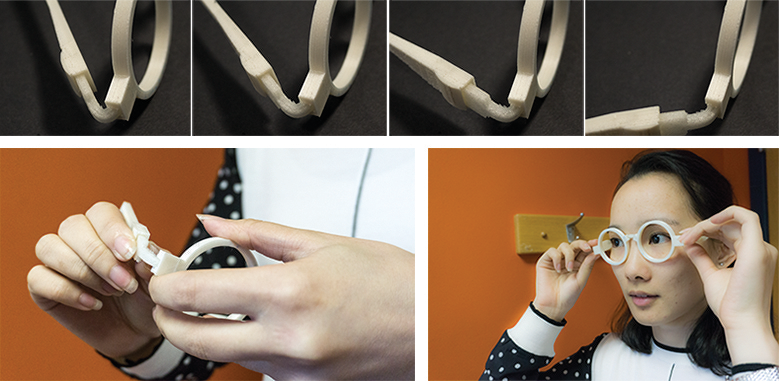
\includegraphics[width=0.75\textwidth]{figures/glasses}
  \caption{Inserting wire makes adjustable hinges for this pair of Harry Potter glasses.}~\label{fig:glasses}
\end{figure}

\textbf{Density} A Bulbasaur phone stand\footnote{\url{https://www.thingiverse.com/thing:1726679}} designed for earlier devices is too light to stably hold large smart phones (e.g., iPhone 8 Plus). We embed three nuts to put more weight on its base, leveraging their higher density (Figure~\ref{fig:phone_stand}). Please see our accompanying video figure for a demo.

\begin{figure} [h]
  \centering
  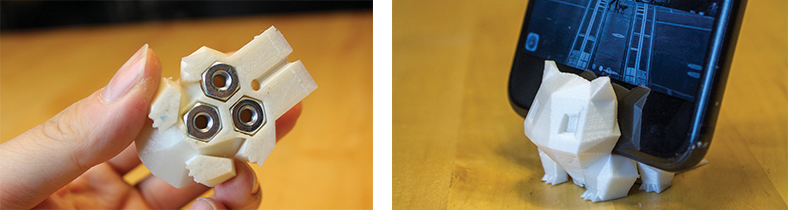
\includegraphics[width=0.75\textwidth]{figures/phone_stand}
  \caption{Embedding higher density nuts adds weight to stabilize this printed stand for large smart phones.}~\label{fig:phone_stand}
\end{figure}

\textbf{Softness} People with hand injuries or motor impairment might have difficulty holding hand tools. Similar to creating adaptations \cite{chen2016reprise}, we can integrate embeddables like a kitchen sponge to create a softer grip of a wrench (Figure~\ref{fig:wrench}), which also tightens the grip as sponge has higher friction coefficient due to its porousness.

\begin{figure} [h!]
  \centering
  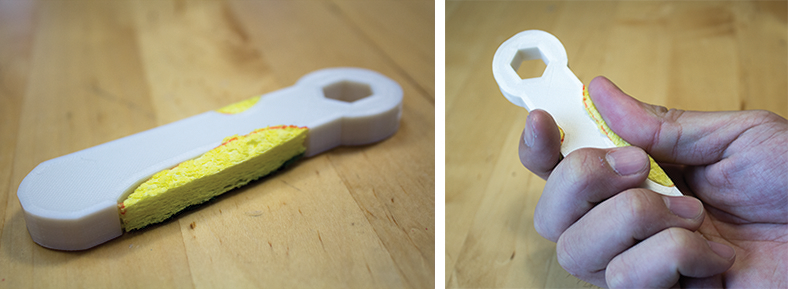
\includegraphics[width=0.75\textwidth]{figures/wrench}
  \caption{Embedding sponge softens and tightens the grip of this printed wrench.}~\label{fig:wrench}
\end{figure}

\textbf{Friction} As another example of friction, in Figure~\ref{fig:door_stop}, a regularly 3D printed door stop would slip on a carpet. Embedding a piece of rubber sheet to replace its bottom increases friction and makes it a functional door stop. Further, rubber also has nice \textbf{abrasion resistance}, making the door stop more durable.

\begin{figure} [h!]
  \centering
  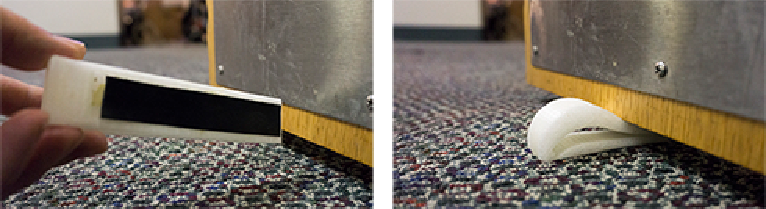
\includegraphics[width=0.75\textwidth]{figures/door_stop}
  \caption{Embedding a piece rubber to make a functional door stop.}~\label{fig:door_stop}
\end{figure}

\textbf{Roughness} As shown earlier in Figure~\ref{fig:fig1}c, embedding a piece of sand paper adds roughness and makes a simple sander.

\textbf{Flexural strength} As shown earlier in Figure~\ref{fig:fig1}b, a screw adds flexural strength to a 3D printed peg board hook, as it approximates replacing part of the hook with a stronger material. Embedding a wire straightened from a paper clip into a spoon avoids snapping during breakage, as snapping could be dangerous to the user (Figure~\ref{fig:spoon}).

\begin{figure} [h!]
  \centering
  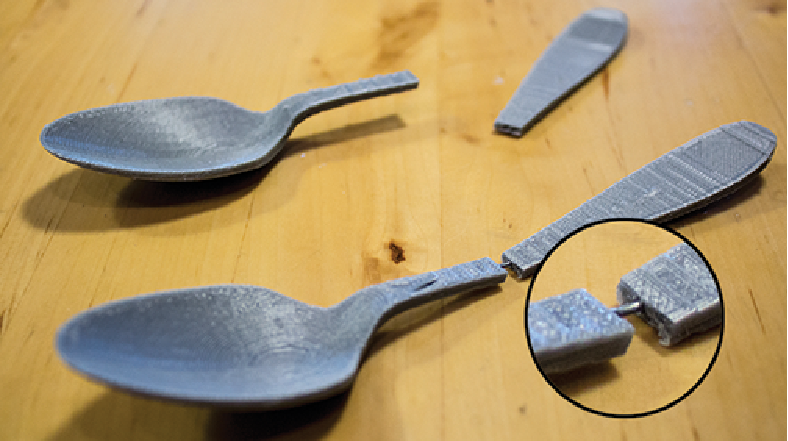
\includegraphics[width=0.75\textwidth]{figures/spoon}
  \caption{Embedding wire straightened from a paper clip into a spoon avoids snapping, which could be dangerous to the user during breakage. Please also see our accompanying video figure.}~\label{fig:spoon}
\end{figure}

\textbf{Malleability} As shown earlier in Figure~\ref{fig:fig1}d, embedding wax (carved from a candle) into an a spoon handle allows users to sand it to a custom shape that the fingers can grip comfortably. 

\textbf{Optical properties} As shown in Figure~\ref{fig:lamp_shade}, for a 3D printed lamp shade, embeddables (e.g., transparent marbles) can add rich optical properties, e.g., making part of the lamp shade more translucent, refracting light to brighten the upper part that is otherwise a bit dark. 

\begin{figure} [h!]
  \centering
  
\includegraphics[width=0.75\textwidth]{figures/lamp_shade2}
  \caption{Embedding clear marbles into a lamp shade makes it more translucent, and can also refract light to brighten the upper part.}~\label{fig:lamp_shade}
\end{figure}

\textbf{Thermal properties} Some embeddables have high heat conductivity, such as coins, which can be used to create simple heat sinks on a printed laptop stand (Figure~\ref{fig:laptop_stand}). Others can insulate, such as silicone oven mitts, which can be used to make printed utensils (e.g., tongs) heat resistive (Figure~\ref{fig:tongs}).

\begin{figure} [h!]
  \centering
  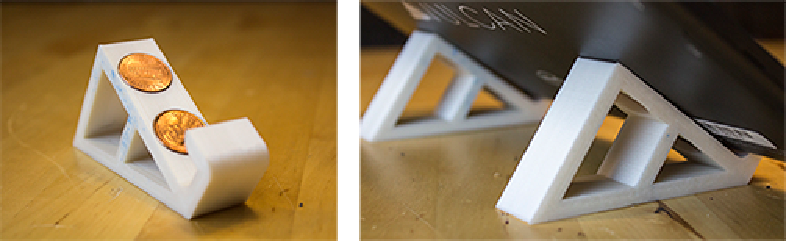
\includegraphics[width=0.75\textwidth]{figures/laptop_stand}
  \caption{Embedding coins to laptop stands creates a heat sink.}~\label{fig:laptop_stand}
\end{figure}

\begin{figure} [h!]
  \centering
  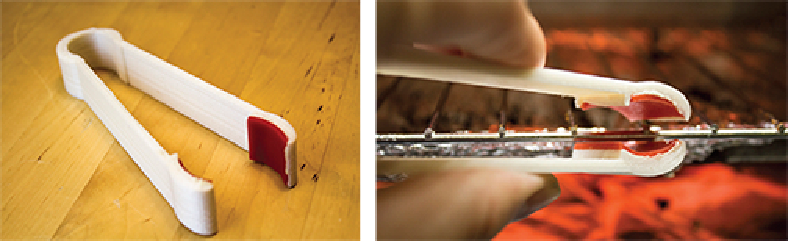
\includegraphics[width=0.75\textwidth]{figures/tongs}
  \caption{Embedding scraps cut from a silicone oven mitt into a pair of tongs makes it possible to be used with hot objects.}~\label{fig:tongs}
\end{figure}

Having demonstrated a series of embeddable results, the next few sections  describe the technical approaches underpinning the design and fabrication process.


\begin{figure} [h!]
  \centering
  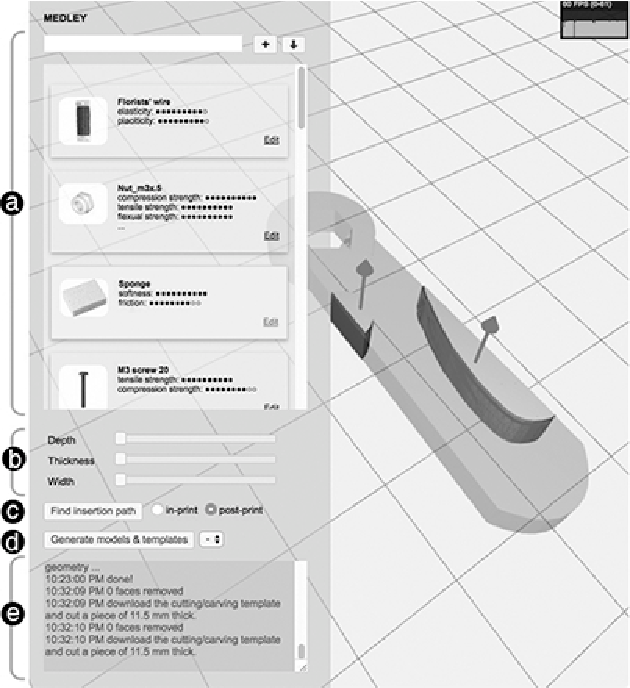
\includegraphics[width=0.75\textwidth]{figures/tool_overview}
  \caption{Overview of Medley, the computational tool that supports the library of embeddables, from searching an embeddable by material properties (a), to interactively specifying its geometry and placement (b), to finding an optimal insertion path (c), and to generating fabrication-ready model (d) and instructions for the crafting process (e).}~\label{fig:tool_overview}
\end{figure}

\section{Overview of Design and Fabrication Process}
We develop Medley--a computational tool to support the design and fabrication of objects with embeddables (Figure~\ref{fig:tool_overview}). A design object (e.g., a wrench) can be imported to the tool. As shown in Figure~\ref{fig:tool_overview}a, the library lists each embeddable  as a card that contains a thumbnail image, a name, and a short list of material properties. Typing in the search bar finds a specific embeddable, as it dynamically filters  embeddables that match the input keywords. 

Clicking on an embeddable highlights and selects it (Figure~\ref{fig:tool_overview}a), and applies it to the subsequent actions, which we briefly describe here and discuss in further details in the next few sections:

\begin{itemize}
	\item \textbf{Specifying the geometry of embeddables}. Given the DOW of an embeddable, Medley enables the creation of custom embeddable geometry by directly sketching on the design object, and manipulating its DOW using simple slider widgets (Figure~\ref{fig:tool_overview}b).
	\item \textbf{Finding optimal paths to insert embeddables}. Once an embeddable is created and placed into the design object, Medley searches for an optimal insertion path with minimal removal of the design object's original volume. It supports inserting the embeddable both during and after the printing process (Figure~\ref{fig:tool_overview}c).
	\item \textbf{Generating guides for crafting embeddables}. Finally Medley generates a fabrication-ready 3D model with carved out insertion path, as well as guides to cut embeddables into specified shapes (Figure~\ref{fig:tool_overview}de).
\end{itemize}


% \section{Medley: A Design Tool for Embeddables}
% drag and drop an object

\section{Specifying the Geometry of Embeddables}
Once an embeddable is selected, the next step is to specify its geometry \textit{in vivo} on a design object, such as the position and orientation of a fixed-shape embeddable ($DOW=0$), or the shapes for workable embeddables ($DOW>0$).

\begin{figure} [t]
  \centering
  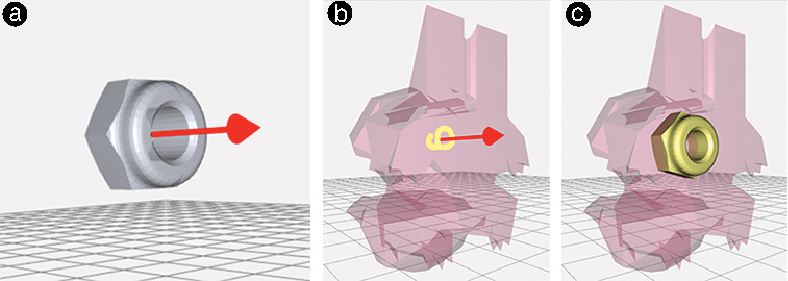
\includegraphics[width=0.75\textwidth]{figures/spec_dow0}
  \caption{Specifying the geometry of a DOW=0 embeddable (e.g., a nut) by `drawing' it on a design object (b), which aligns its pre-computed principal axis (a) with that of the sketched points' (bc).}~\label{fig:spec_dow0}
\end{figure}

One challenge here is that different $DOW$s constrains how an embeddable can be created in different ways, which could significantly increase the complexity of the interface. As detailed below, Medley addresses this by providing a unified sketch-based input vocabulary that enables simply drawing on the surface of the design object to initiate the placement of the embeddable, or the creation of its shape. A second challenge is aligning an embeddable to certain parts of the design object. This task could be cumbersome if only using translation/rotation/scaling operations in the Cartesian system, as the X/Y/Z coordinates do not necessarily align with the object's geometry. To address this, Medley leverages the design object's geometry as a constraint to simplify the editing and transformation task, reducing the variables from nine (translating/rotating/scaling with respect to each of X/Y/Z) to at most three (depth, width and thickness). Below we detail our approaches to tackle these two challenges.

$\mathbf{DOW=0} \;$ For a fixed-shape embeddable, we pre-compute its principal axis $\mathbf{n_e}$---an axis that represents the global orientation of an object---by first fitting all its vertices to a plane using Singular Value Decomposition (SVD) \cite{strang2011introduction}, and then taking the plane's normal as $\mathbf{n_e}$ (Figure~\ref{fig:spec_dow0}a). As one sketches on the design object, we compute the principal axis $\mathbf{n_s}$ from the sketch points (Figure~\ref{fig:spec_dow0}b). First, we convert the sketch points $\{P_0,~P_1, ~... ~P_N\}$ to a polyline $L$. If $L$ is closed (i.e., a forming a polygon), we apply the similar SVD method; if $L$ is open, we compute $\mathbf{n_s}$ as ${1 \over {N-1}} \sum^N_{i=1}(P_i - P_0)$
%, where $P_i$ is the $i^{th}$ sketch point. 
We then position the embeddable at the centroid of the sketch $P_c$, and orient it by aligning $\mathbf{n_e}$ to $\mathbf{n_s}$ (Figure~\ref{fig:spec_dow0}c).

\begin{figure} [t]
  \centering
  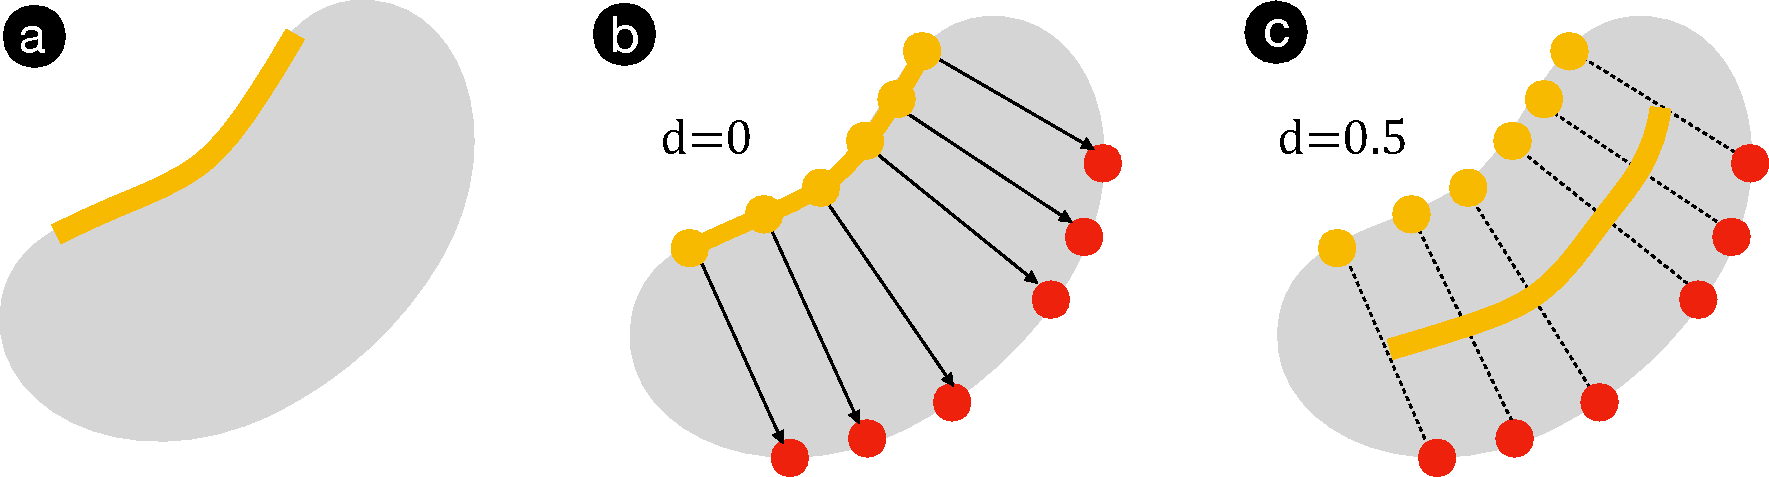
\includegraphics[width=0.75\textwidth]{figures/control_points}
  \caption{Top view of `pushing' an embeddable to a design object: after sketching a to create the geometry (a), each sketch point raycasts along the reversed direction of its normal to find another control point (b), and by interpolating pairs of these points we can `push' in an embeddable, which is driven by a depth value \textit{d} between 0 and 1.}~\label{fig:control_points}
\end{figure}

Once the embeddable is aligned and placed on the surface at $P_c$, we can push it into the design object by adjusting the `depth' slider. To enable this interaction, we first raycast from $P_c$ along the reverse of its normal, which will hit $Q$ on the other side of the design object. We use $P_c$ and $Q$ as control points: given a depth ratio $d$ read from the slider, we position the embeddable at $(1-d)P_c + dQ$. This approach is applied to all the embeddables with different DOW's. A more general illustration of the process is shown in Figure~\ref{fig:control_points}.
% To enable this interaction, we use two sets of control points. The first set $C_1$ consists of users' sketch points, and the second set $C_2$ is obtained by raycasting from each vertex in $C_1$ along the reverse of its normal, which will hit the other side of the design object. The depth of $e_0$ is computed as a linear interpolation

$\mathbf{DOW=1}$ enables two ways of creating a `tunnel' for putting in an embeddable: continuously drawing a freeform path (Figure~\ref{fig:spec_dow1}ab) and discretely clicking at points that consecutively connect to one another (Figure~\ref{fig:spec_dow1}cd). Both actions return a polyline $L$. To make sure the material can be inserted into the tunnel, we straighten $L$ so that it does not go under the embeddable's bend radius limit $r_e$. In particular, we iteratively evaluate each three consecutive vertices on $L$, and fix those whose curving radius is smaller than $r_e$. We then extrude geometry along the `straightened' $L$ using a circular cross section with the embeddable's radius.

Similar to $DOW=0$, it is possible to push the embeddable into the design object using the `depth' slider (Figure~\ref{fig:spec_dow1}f). This is implemented by creating two control points for each vertex along $L$ and interpolating them with the given depth ratio.


$\mathbf{DOW=2, 3} \;$ There are two ways to create geometry for a $DOW=2$ embeddable ($e_2$), both of which can be easily extended to a $DOW=3$ embeddable ($e_3$): 

\begin{itemize}
	\item Drawing a freeform \textit{open} line $L$ (Figure~\ref{fig:spec_dow2a}), which is similar to the input for $DOW=1$. However, instead of extruding a `tunnel', we expand the polyline $L$. First we compute a fitting plane using SVD based on all the sketch points as well as their normals (one such normal is obtained by interpolating the vertex normals of the face that contains a sketch point). Then as shown in Figure~\ref{fig:spec_dow2a}, we expand $L$ bi-directionally along each sketch point's normal (Figure~\ref{fig:spec_dow2a}b), which creates a plane cutting into the design object (Figure~\ref{fig:spec_dow2a}c); next, we extrude the plane bidirectionally along its own normal (Figure~\ref{fig:spec_dow2a}d), thus creating a full geometry representing the embeddable (Figure~\ref{fig:spec_dow2a}e).

	The amount of these two expansions corresponds to thickness and width, respectively. While $DOW=2$ embeddables have fixed thickness and can only vary width, $DOW=3$ embeddables allows for adjustable thickness. Further, both can adjust their depth using the aforementioned control point approach applied on $DOW=1$.
	
	\item Drawing a freeform \textit{closed} line (or pressing `shift' to automatically close an open line) indicates a polygon $S$ rather than a polyline (Figure~\ref{fig:spec_dow2b}a). To create the embeddable geometry, we first retrieve a set of neighoring faces from the design object within a certain geodesic distance from the center of the polygon (Figure~\ref{fig:spec_dow2b}b). We then re-tessellate these faces: for a given face $f$, we retain it if its vertices are all in $S$, and remove it if they are all outside of $S$; otherwise we retessellate and include the part of $f$ that intersects with $S$ (Figure~\ref{fig:spec_dow2b}cd).

	These new tessellated faces create the top side of the embedded geometry (Figure~\ref{fig:spec_dow2b}e). Next, we again obtain a set of control points from raycasting, which create the bottom side of the embeddable geometry. We then add the lateral area between the two sides to finish the whole geometry.

	Depth and thickness are adjustable (with thickness only applicable to $DOW=3$) using the top and bottom vertices as control points.
\end{itemize}

\begin{figure} [t]
  \centering
  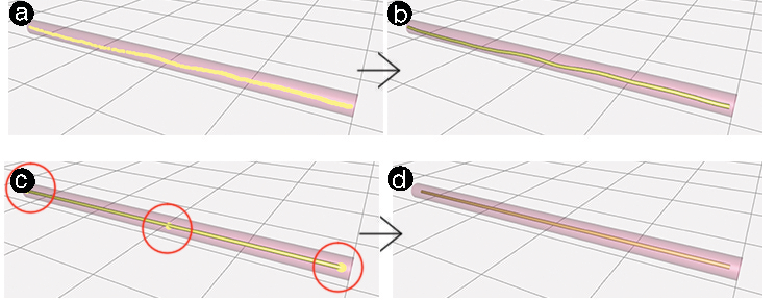
\includegraphics[width=0.75\textwidth]{figures/spec_dow1}
  \caption{Specifying the geometry of a DOW=1 embeddable (e.g., a wire) by drawing a continuous line (ab) or clicking at discrete points (cd).}~\label{fig:spec_dow1}
\end{figure}

To summarize, an embeddable's geometry can be created using a unified technique---sketching on the design object. In other words, selecting an embeddable is similar to choosing a type of paint brush that is subsequently applied to the sketching action. Medley handles the geometric and material details (e.g., DOW, bend radius) while keeping the sketch-based interaction consistently to the minimum across different types of embeddables (e.g., drawing one single stroke). Further, to address the challenge of alignment, Medley uses the design object's geometry as constraint so that the positioning and orienting of an embeddable is in relation to the design object's own geometric and spatial properties, such as using points intersected with the design object as control points to position the depth of an embeddable.



\begin{figure*} [h]
  \centering
  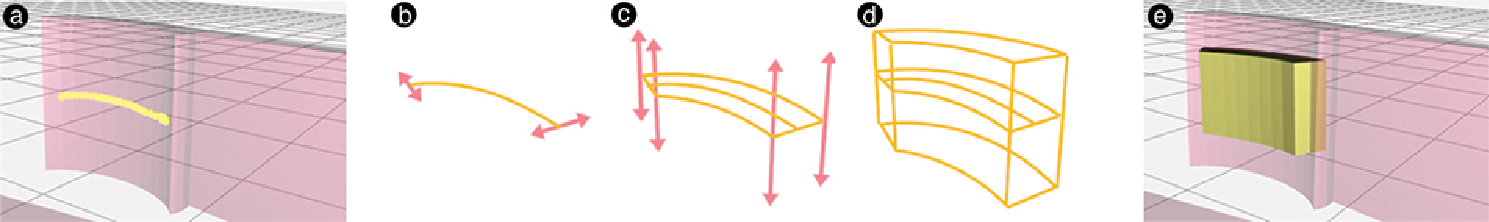
\includegraphics[width=1\textwidth]{figures/spec_dow2a}
  \caption{Specifying the geometry of a DOW=2, 3 embeddable by drawing an open freeform line (a), which is then expanded into a 3D shape with controllable thickness and width (b$\rightarrow$e).}~\label{fig:spec_dow2a}
\end{figure*}

\begin{figure*} [h]
  \centering
  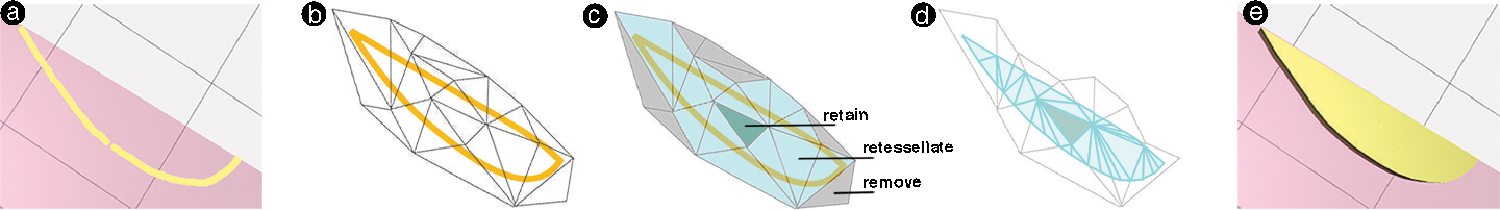
\includegraphics[width=1\textwidth]{figures/spec_dow2b}
  \caption{Specifying the geometry of a DOW=2, 3 embeddable by drawing an (automatically) closed line (a), which is then retessellated to a surface extrudable into a 3D shape (b$\rightarrow$e).b}~\label{fig:spec_dow2b}
\end{figure*}

\section{Finding Optimal Paths to Insert Embeddables}
% \subsection{Guidance for Cutting or Carving Embeddables }
Once an embeddable's geometry is specified, the next step is to find ways to insert it into the design object. In terms of timing, an embeddable can be inserted while printing the design object (in-print), or after the printing is finished (post-print). We can also choose whether the insertion process allows for deformation of the embeddable. For example, inserting a wire causes it to undergo bending while being inserted; inserting a nail, on the other hand, should require no deformation. In our current system, we only consider deformational insertion for $DOW=1$ with high stiffness (e.g., metal wires but not threads or strings). % should also consider stiffness?
Figure~\ref{fig:insertion} summarizes the $2\times2=4$ ways of inserting embeddables.

\begin{figure} [h]
  \centering
  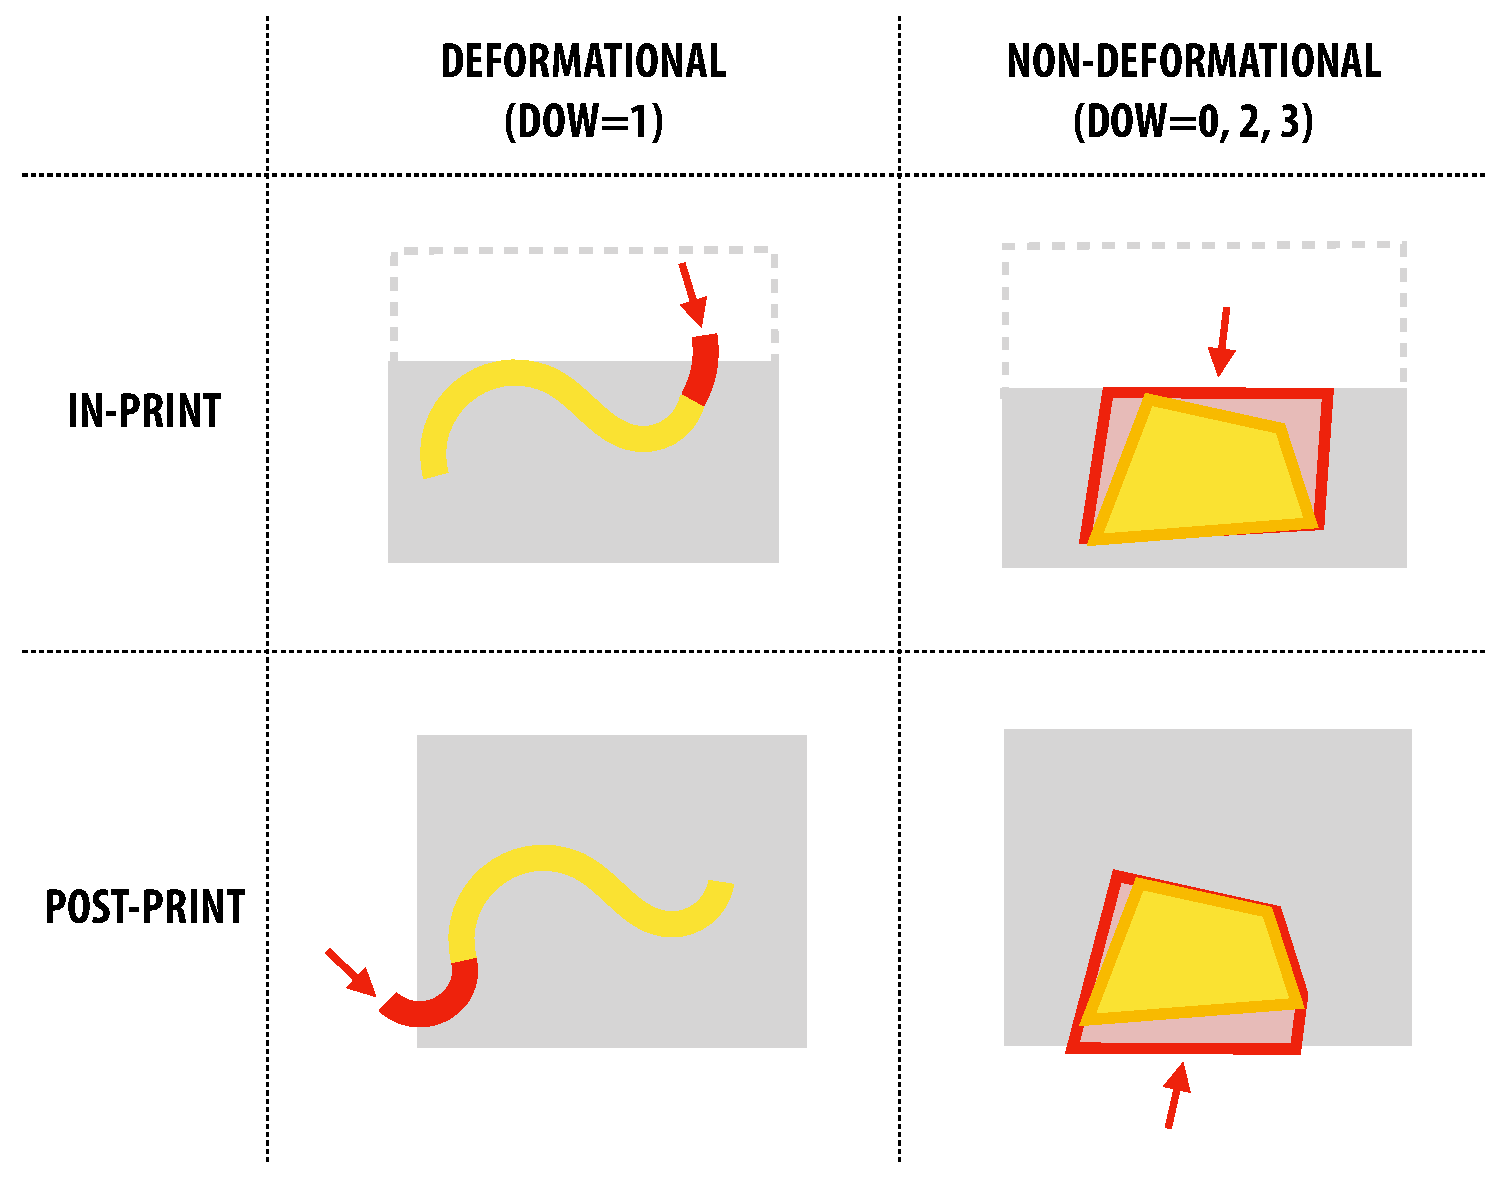
\includegraphics[width=0.7\textwidth]{figures/insertion}
  \caption{A 2x2 space of inserting embeddables that considers {\em(i)} whether insertion occurs during or after printing the design object; and {\em(ii)} whether the embeddables undergo deformation during insertion.}~\label{fig:insertion}
\end{figure}

Below we provide details for each of these scenarios, in particular how Medley searches for the optimal path by minimizing the amount of the design object that needs to be removed in order to insert the embeddable.

\subsection{Deformational Insertion of DOW=1 Embeddables}
For $DOW=1$ we can create a polyline `tunnel' $L$ to contain the embeddable inside the design object. To generate a path for inserting the embeddable, we extend $L$ to the nearest surface. Medley computes such paths for both in-print and post-print insertions, and provides a solution with minimized path length. The first column of Figure~\ref{fig:insertion} illustrates the follow insertion path finding scenarios.

\textbf{In-print insertion} assumes the entrance of insertion is at the layer where the print job will be paused and the embeddable inserted. First we orient the design object to a user-specified printing direction. Next, along that direction we compute the pausing point, which is a point on $L$ with the highest value when projected on the printing direction. Now, we can extend either one of $L$'s end points to the layer defined by the pausing point. As shown in Figure~\ref{fig:dow1_insertion}, we compute the tangent vector of an end point, and generate a circular extension path whose radius equals the embeddable's bend radius. Amongst all such possible paths in 3D space, we discard those that cannot reach the pausing layer, and for those that can, we search for the one with the shortest length. We perform this process twice, once for each end point, and obtain the shortest path to insert the embeddable at the pausing layer.

\begin{figure} [h]
  \centering
  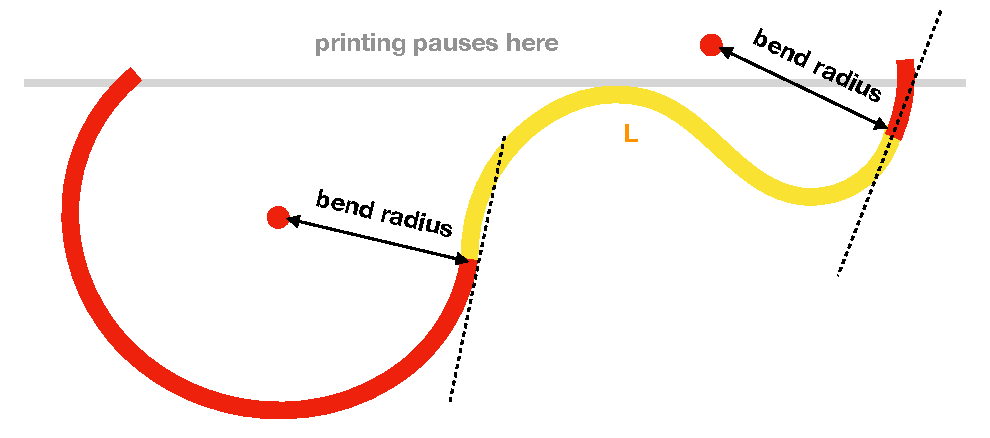
\includegraphics[width=0.7\textwidth]{figures/dow1_insertion}
  \caption{Finding an optimal insertion path for DOW=1 by extending each of the end points along its tangent vector, and along a circular path of radius equal to the bend radius of the material. We compute and search for the shortest amongst all possible paths.}~\label{fig:dow1_insertion}
\end{figure}

\textbf{Post-print insertion} We perform a similar shortest extension path searching process, except the destination is on the surface of the design object, rather than a horizontal sliced plane.


\subsection{Non-deformational Insertion of DOW=0, 2, 3 Embeddables}
For non-deformational insertion, the insertion path needs to accommodate a sliding volume of the embeddable's geometry (e.g., without undergoing bending). Given a user-defined printing direction, Medley finds a insertion path that minimizes such volume.
% optionally, it can also create geometry to fill in the path once the embeddable is inserted, avoiding leaving a cavity inside the design object.

\textbf{In-print insertion.} Similar to the deformational case, we first compute the pausing layer. Next, we perform a step-wise (step=5$^{\circ}$) search across possible insertion directions at the pausing layer. For a given insertion direction $\theta$, we compute the minimum volume of the design object that needs to be removed in order for the embeddable to be inserted. To compute this volume, we first discretize the embeddable based on the printing layer height $\Delta h$: given $\theta$, the to-remove volume can be discretized into $N$ layers, each perpendicular to $\theta$ and has a height of ${\Delta h} / \cos(\theta)$ as shown in Figure~\ref{fig:dow023_insertion}. 

\begin{figure} [h]
  \centering
  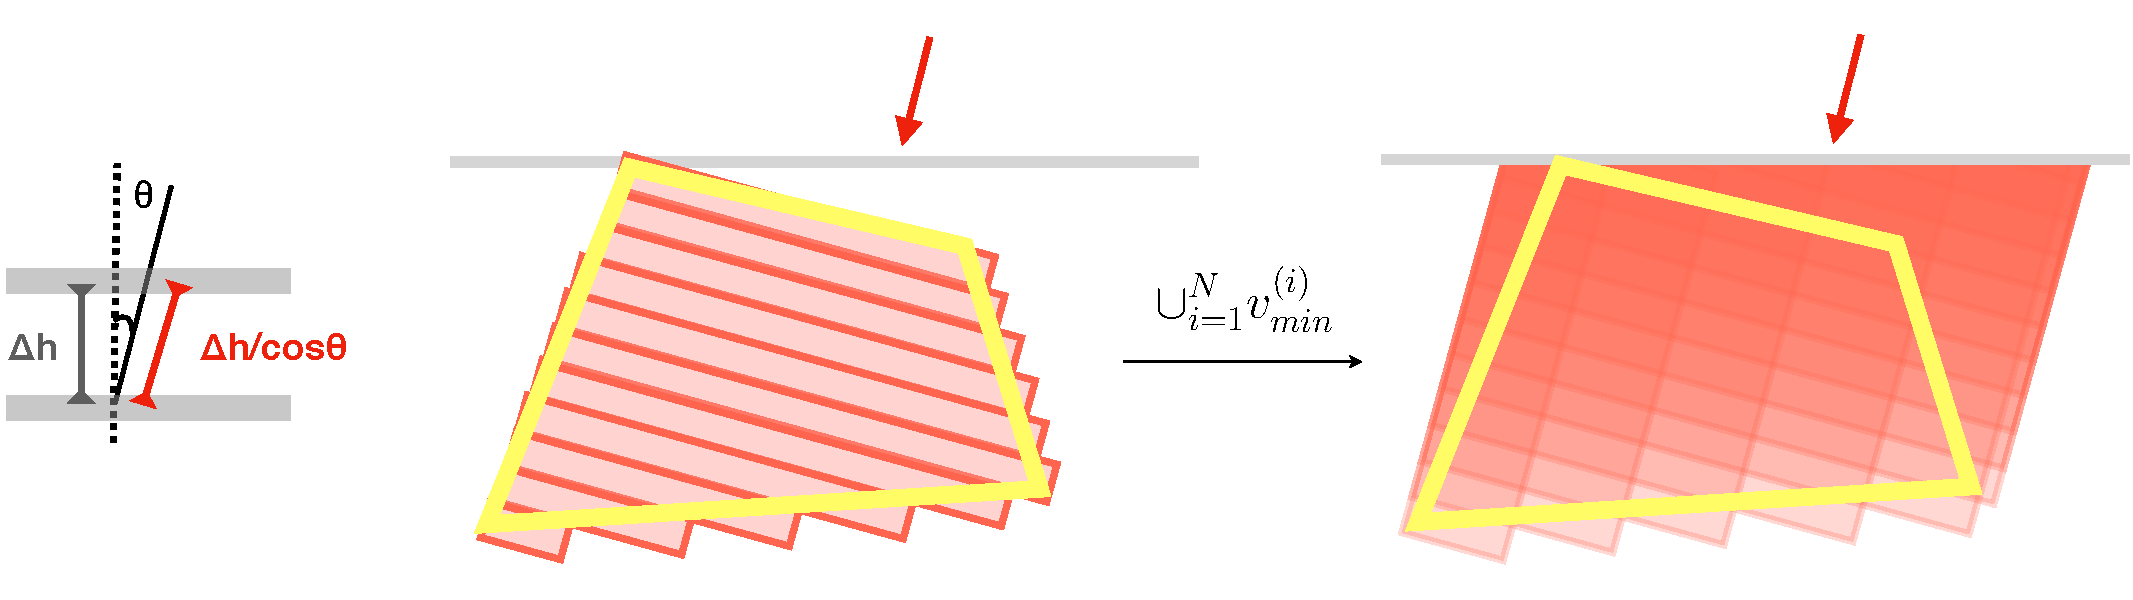
\includegraphics[width=0.7\textwidth]{figures/dow023_insertion}
  \caption{Finding an optimal insertion path for DOW=2, 3: for a given insertion direction $\theta$, we compute the minimum volume that needs to be removed in order to insert an embeddable; we then search step-wise across possible insertion directions to find one with the minimum to-remove volume.}~\label{fig:dow023_insertion}
\end{figure}

The minimum volume of the entire N-layered embeddable can be computed as $V_{min} = \cup_{i=1}^N{v_{min}^{(i)}}$, where
% \sum_{i=1}^N{v_{min}^{(i)} \cup V^{(i-1)}_{min}}$, where 
$v_{min}^{(i)}$ is the minimum volume for inserting the $i^{th}$ layer, which can be obtained by sliding (or extruding) that layer from its position along $\theta$ until its entirety is outside of the (partially printed) design object; $\cup$ is a union operator.
%and removes the parts where they overlap. 
As shown in Figure~\ref{fig:dow023_insertion}, the minimum volume for inserting an embeddable is the minimum volume for inserting each of its layers at their corresponding position.
Our search process finds $\theta_{min}$ with the minimum $V_{min}$ amongst all possible insertion directions.


\textbf{Post-print insertion.} We perform a similar search process, except for each $\theta$ the volume for insertion needs to start from the surface of the design object, rather than a pausing layer.

% One problem of non-deformational insertion is it often leaves a `gap' once the embeddable is inserted (figure xx). To mitigate this problem, we compute and generate

\section{Generating Guides for Crafting Embeddables}
As a final step, we perform a Boolean operation, subtracting the geometry of the insertion path from the design object. As shown in Figure~\ref{fig:cap}, one problem is that this operation will generally leave an `hole' on the object's surface (for post-print insertion), or in its inner structure (for in-print insertion). To mitigate this problem, we generate a `cap' that can be 3D printed to fill in the hole once an embeddable is inserted. Figure~\ref{fig:cap_printing} shows a example of embedding a nut and a cap (printed in advance) during the printing process.

For non-deformational insertion ($DOW=0, 2, 3$), we first compute the convex hull of the embeddable, and then subtract it from the geometry of the insertion path to obtain the cap. This approach, however, does not work for deformational insertion, as the printing material might not have the bend radius to allow it to be inserted into the hole. Second, to insert a thin wire/rod, one often needs to cut it longer than the insertion path in order to hold and push it in, which will already fill the hole once inserted. Given these considerations we currently do not to add a cap to deformational insertions.

\begin{figure} [h]
  \centering
  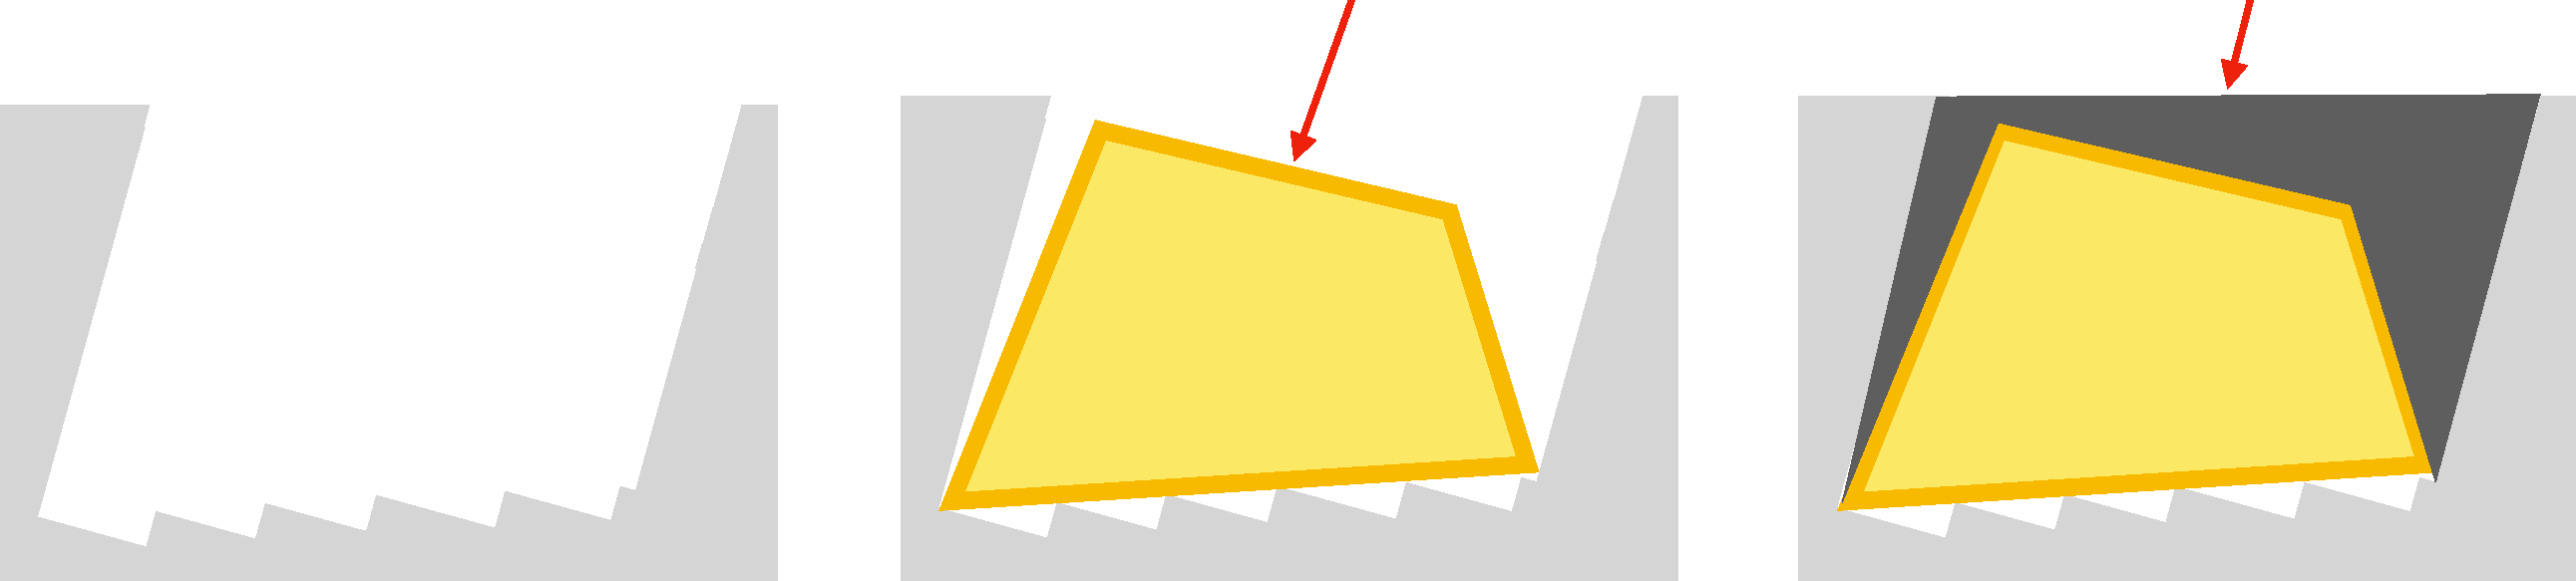
\includegraphics[width=0.75\textwidth]{figures/cap}
  \caption{Generating a cap to fill up empty space created by removing volume for the insertion path}~\label{fig:cap}
\end{figure}

\begin{figure*} [h]
  \centering
  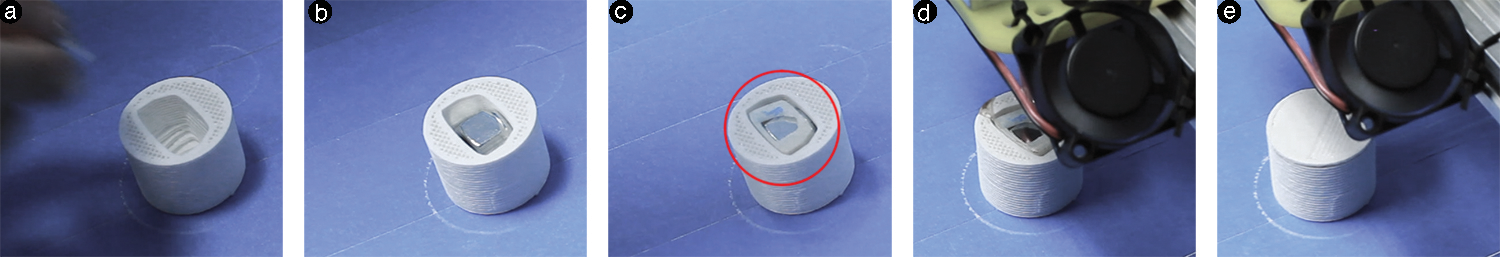
\includegraphics[width=1\textwidth]{figures/cap_printing}
  \caption{Demonstration of inserting a cap during the printing process: an embeddable (a nut) is inserted (ab), and then a cap (c), after which the printing continues (d) and finishes (e).}~\label{fig:cap_printing}
\end{figure*}

Embeddables with non-zero $DOW$ also needs to be cut or carved to match the geometry specified in the tool. We generate guides to aid this crafting process. For $DOW=1$, we output the length $l$ of the embeddable by summing up the distances of the segments on the polyline drawn by the user. For $DOW=2, 3$, there are two types of geometry. One is extruded from a polyline, and thus can be obtained by cutting or carving a $l \times w \times t$ piece, where $l$, $w$ and $t$ correspond to the drawn length, the adjustable width, and the embeddable's material thickness (fixed for $DOW=2$, adjustable for $DOW=3$), respectively. The other type of geometry is extruded from a polygon. We generate a thin piece of the polygon that can be printed and then used as templates for cutting/carving a piece of embeddable with $t$ thickness. For example, to craft the embeddables for the wrench (Figure~\ref{fig:wrench}), we printed two templates alongside the wrench (Figure~\ref{fig:template}a). As shown in Figure~\ref{fig:template}b, we then used the templates to trace the designed profile on a sponge and then carved out the embeddable with the thickness informed by Medley's output (Figure~\ref{fig:tool_overview}e).

\begin{figure} [h]
  \centering
  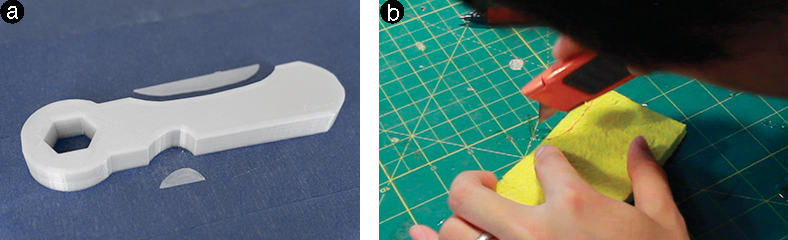
\includegraphics[width=0.75\textwidth]{figures/template}
  \caption{For freeform custom embeddable geometry, we generate printable templates to assist the crafting process: in the case of making the soft wrench handle, we can use the printed templates to trace the embeddable's shapes on a sponge before carving them out.}~\label{fig:template}
\end{figure}

We apply two strategies to attach embeddables to printed objects. First, having calibrated our 3D printers, we slightly scale the generated insertion path (between 0.5 and 1 mm smaller) to press fit the embeddables, such as fitting a wire into a `noodle', and fitting a piece of sand paper into the slot on a printed sander (Figure~\ref{fig:fig1}c). In other cases where the objects and the embeddables cannot press into one another, we use a versatile and temperature resistant adhesive\footnote{Currently we use Gorilla Original Glue: \url{http://www.gorillatough.com/gorilla-glue}}.

%\pagebreak


,
In this section we discuss outstanding issues, existing limitations and future work for embeddables.

\textbf{Extending the current library of embeddables}
Our embeddable library is extensible. As shown in Figure~\ref{fig:tool_overview}, clicking `Edit' on each embeddable card brings up a dialog for editing the embeddable. We can change the basic information, such as clicking the name to edit it, or dragging a new image to the dialog to update the thumbnail. More importantly, one can specify information related to material properties. The first step is to select the $DOW$, based on which the dialog further request additional information, such as a 3D model for $DOW=0$ object, radius for $DOW=1$ (e.g., radius of a wire), thickness for $DOW=2$ (e.g., thickness of a sheet), and minimum bend radius for $DOW \in \{1, 2\}$ (e.g., how much a wire or a sheet can be bent).
% - selection
Using the a similar dialog, we can also add a new embeddable to the library.

% \begin{figure}
%   \centering
%   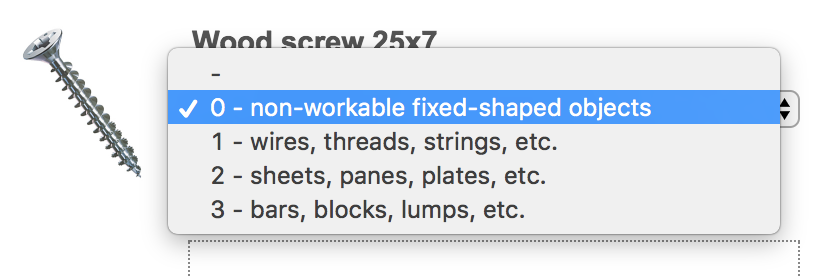
\includegraphics[width=0.9\textwidth]{figures/spec_workability}
%   \caption{specifying workability}~\label{fig:spec_workability}
% \end{figure}

% - search

% Next, we demonstrate using the selected embeddable as a `paint brush' to specify where and how to embed it into a 3D object.

% \begin{figure}
%   \centering
%   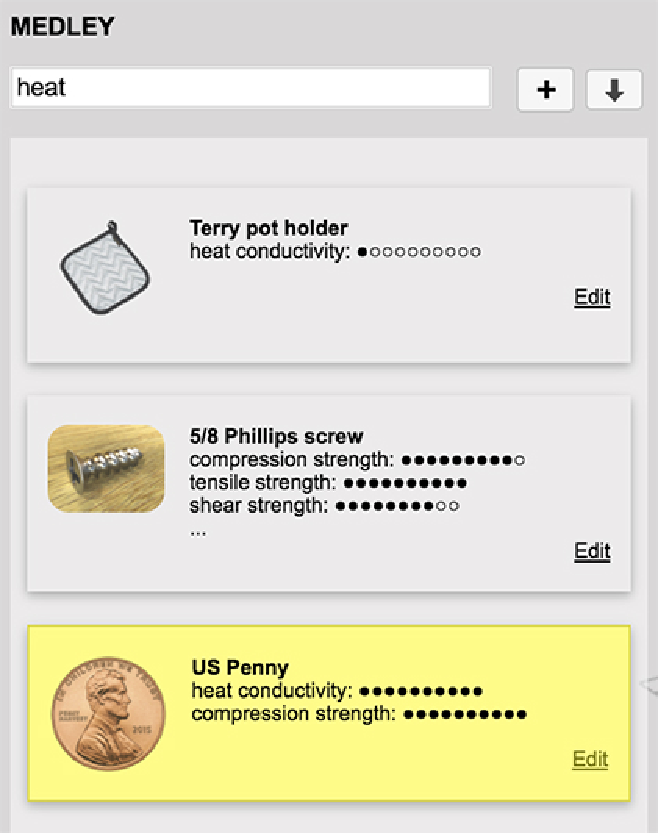
\includegraphics[width=0.5\textwidth]{figures/search_library}
%   \caption{searching in library}~\label{fig:search_library}
% \end{figure}
\textbf{Guidance for quantifying and comparing embeddables}
Currently our library employs a simple rating approach (scale 1 to 10) to quantify the material properties of embeddables, which enables searching for specific embeddables with a target property. As the library grows larger, it would be useful to compare material properties across embeddables, and sort the search results accordingly. One possible direction for future work is to employ \cite{yumer2015semantic}'s method, using the crowd to perform pair-wise comparison for a given material property, based on which a ranking can be computed across all embeddables. Further, we also would like to explore ways to inform users of different material properties and provide more support for them to understand and explore the usage of different embeddables.

\textbf{Limitations of workability and insertion}
While our library and fabricated examples demonstrate a wide range of embeddables, there are objects that cannot be used as embeddables due to a lack of workability or difficulty with insertion. For example, a bike spoke has a nice combination of tensile and compression strengths, and has a small dimension to fit in thin structures; however, it is difficult to cut without specialized tools. Our future work plans to provide a list of tools, which can be incorporated into the library, as a way to inform users how to cut or carve a particular embeddable. Some objects are easy to cut, but much more difficult to insert into a printed design. For example, carbon fibre has great structural properties and has been used in industry for strengthening components such as bike frames or airplane turbines. However, a single thread of carbon fibre is fairly soft and very difficult to insert into a `tunnel' in ways similar to inserting a metal wire. In the future we plan to develop ways to insert such soft embeddables (e.g., perhaps by extending \cite{rivera2017stretching}'s approach with fabric).

% <<<<<<< HEAD
 \textbf{Simulation to inform embeddable choice and design}
 While our library and tool allow people to explore and design with different embeddables, as future focus we should also provide more guidance on: {\em(i)} what are the existing problems of the design, {\em(ii)} what embeddables can be used to solve or mitigate such problems, and {\em(iii)} once inserted whether an embeddable has improved the design. 
%As a first step, we have developed and integrated a finite element analysis (FEA) [ref] module for stress analysis, simulation and visualization. This enables specifying forces that are applied on a object, see the distribution of stress and identfy the weak parts of the design. As different embeddables are generated and inserted, the simulation updates to show whether and how the stress distribution has improved. In the future we plan to experiment with more simulation modules, as well as providing ways for other developers to plug in their own simulations as components to the design tool.

\textbf{Automatically suggesting and generating designs}
Even with simulation, it still requires manually choosing and applying embeddables that are selected from a potentially large library. In the future we will experiment with ways to automatically generate design suggestions based on the input object and problem description (e.g., ``increasing the strength around this area''), which is similar to approaches demonstrated in prior work \cite{terry2002side}. Further, it is also interesting to search for existing designs from other users that match the current design problem, and also use them to generate more design suggestions.


%\xac{better way to attach embeddables to objects?}